\documentclass{beamer}


\usetheme[progressbar=frametitle]{metropolis}
\usepackage{appendixnumberbeamer}

\usepackage{booktabs}
\usepackage[scale=2]{ccicons}

%\usepackage{pgfplots}
%\usepgfplotslibrary{dateplot}

\usepackage{xspace}
\newcommand{\themename}{\textbf{\textsc{metropolis}}\xspace}

%\setbeamertemplate{footline} % To remove the footer line in all slides uncomment this line
%\setbeamertemplate{footline}[page number] % To replace the footer line in all slides with a simple slide count uncomment this line

%\setbeamertemplate{navigation symbols}{} % To remove the navigation symbols from the bottom of all slides uncomment this line


\usepackage{graphicx} % Allows including images
\usepackage{grffile}
\usepackage{amsmath}
% have to have Mozilla's=Fira Sans} font and XeTeX installed to use full typography.

%----------------------------------------------------------------------------------------
%	TITLE PAGE
%----------------------------------------------------------------------------------------

\title{Alliance Participation and Military Spending}
\date{November 28, 2018}
\author{Joshua Alley}
\institute{Texas A\&M University}


\begin{document}

 \maketitle


%----------------------------------------------------------------------------------------
%	PRESENTATION SLIDES
%----------------------------------------------------------------------------------------


%------------------------------------------------
% Question 
 \begin{frame}[standout]

How does alliance participation affect military spending? 

 \end{frame}



%------------------------------------------------
% This is my point. 
 \begin{frame}{Key Points} 

\begin{enumerate}
\item The conventional wisdom predicts strong alliance commitments decrease military spending in small states, and increase spending in large states.
\pause
\item I find strong alliance commitments \textit{increase} military spending in non-major powers and \textit{do not impact} spending in major powers.
\pause
\item So I consider two alternative arguments.
\end{enumerate}

 \end{frame}

%------------------------------------------------

 \begin{frame}{Relevance}

% put some sort of motivation
Current policy debates emphasize low defense spending by alliance members. 

These debates lack theoretical and empirical context: do most alliances lead to reduced defense spending? 


 \end{frame}


%------------------------------------------------

\begin{frame}{Scholarly Importance: Part 1}

Addresses debate between two sets of expectations:
\pause 

\begin{itemize}
\item \textbf{Force Multiplier}- Alliance participation decreases military spending.
\pause 
\item \textbf{Foreign Entanglement}- Alliance participation increases military spending.
\end{itemize} 


 \end{frame}

%------------------------------------------------

\begin{frame}{Mixed Empirical Results}


\begin{table}[hbt!]
\begin{center}
\begin{tabular}{lccc}
     & Decrease & Increase & Null \\
\hline
Most \& Siverson 1987  &  &  & X \\
Conybeare 1994 & X & &  \\
Diehl 1994 &  & X &  \\
Goldsmith 2003 &  &  & X \\
Morgan \& Palmer 2006 &  & X & \\ 
Quiroz-Flores 2011 &  & X &  \\ 
Digiuseppe \& Poast 2016 & X &  & \\ 
Horowitz et al 2017 &  & X & \\ 
\hline
\end{tabular}
\end{center} 
\end{table}



 \end{frame}

%------------------------------------------------

\begin{frame}{Outline}

\begin{enumerate}
\item Initial Expectations: Alliance Strength
\pause
\item Statistical Analysis
\pause
\item Alternative Arguments
\end{enumerate}


\end{frame}

%------------------------------------------------

\section{Initial Expectations}

%------------------------------------------------

\begin{frame}{Key Principles}

\begin{itemize}
\item Alliances provide security for members.  
\pause
\item Small states depend on larger partners, and sacrifice autonomy for security.
\pause
\item Large states provide security, and gain autonomy. 
\end{itemize}



\end{frame}

%------------------------------------------------

\begin{frame}{Treaty Strength}

Not all alliances are equally valuable. 

\pause

Alliance Treaty Value $= \Delta$ Pr(Support) * Allied Capability:

\pause

Strong/reliable alliance commitments $\uparrow$ Pr(Support)


\end{frame}

%------------------------------------------------

\begin{frame}{Unconditional Alliance Commitments and Spending}

Unconditional alliance commitments provide better security--- reflected in treaty design. 

\pause

\begin{itemize}
\item Small states rely more on their allies. 
\pause
\item Large states increase spending to cover junior partners.  
\end{itemize}


\end{frame}


%------------------------------------------------

\begin{frame}{Predictions}


\begin{quote}
\textsc{Hypothesis 1}: Unconditional alliance participation will be associated with increases in defense spending by major powers. 
\end{quote} 

\pause

\begin{quote}
\textsc{Hypothesis 2}: Unconditional alliance participation will be associated with decreases in defense spending by non-major powers. 
\end{quote} 


\end{frame}

%------------------------------------------------

\section{Empirical Analysis} 

%-----------------------------------------------

\begin{frame}{Research Design}

\begin{enumerate}
\item \textbf{Key Independent Variable}: Binary indicator of Unconditional Alliance. 
\pause
\item \textbf{Base Category}: States with alliances that do not offer military support, and states with no alliances. 
\pause
\item \textbf{Dependent Variable}: Ln(Military Spending) 
\pause 
\item \textbf{Estimator}: Robust Regression. 
\end{enumerate}


\end{frame}

%------------------------------------------------

\begin{frame}{Sample and Controls}

\begin{itemize}
\item \textbf{Sample}: All states: 1816-2007. 
\pause 
\item Divided into two sub-samples: major and non-major power states. 
\pause
\item Lagged DV
\pause
\item \textbf{Controls}: Conditional Military Support, Interstate war, Civil War, Annual MIDs, GDP, POLITY, Cold War, Major Power, Rival military expenditures, ln(ally expend), Average Alliance Size, Avg Democracy Among Allies. 

\end{itemize} 



\end{frame}

%------------------------------------------------

\section{Results}

%------------------------------------------------

\begin{frame}{Impact of Unconditional Military Support on Military Spending} 

\begin{figure}[htbp]
	\centering
		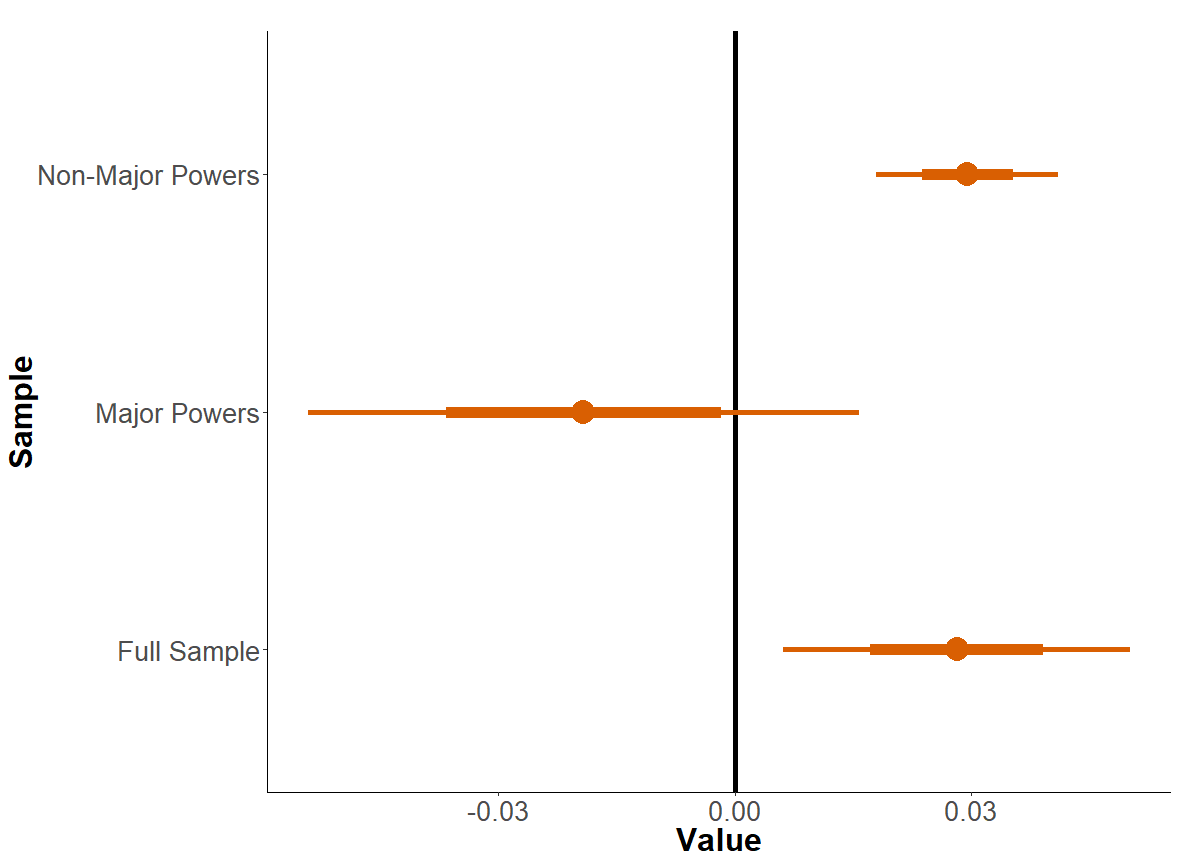
\includegraphics[height=0.90\textheight]{robust-reg-coef.png}
	\label{fig:robust-reg-coef}
\end{figure}

\end{frame}


%------------------------------------------------

\begin{frame}{Dynamic Simulation} 

\begin{figure}
	\centering
		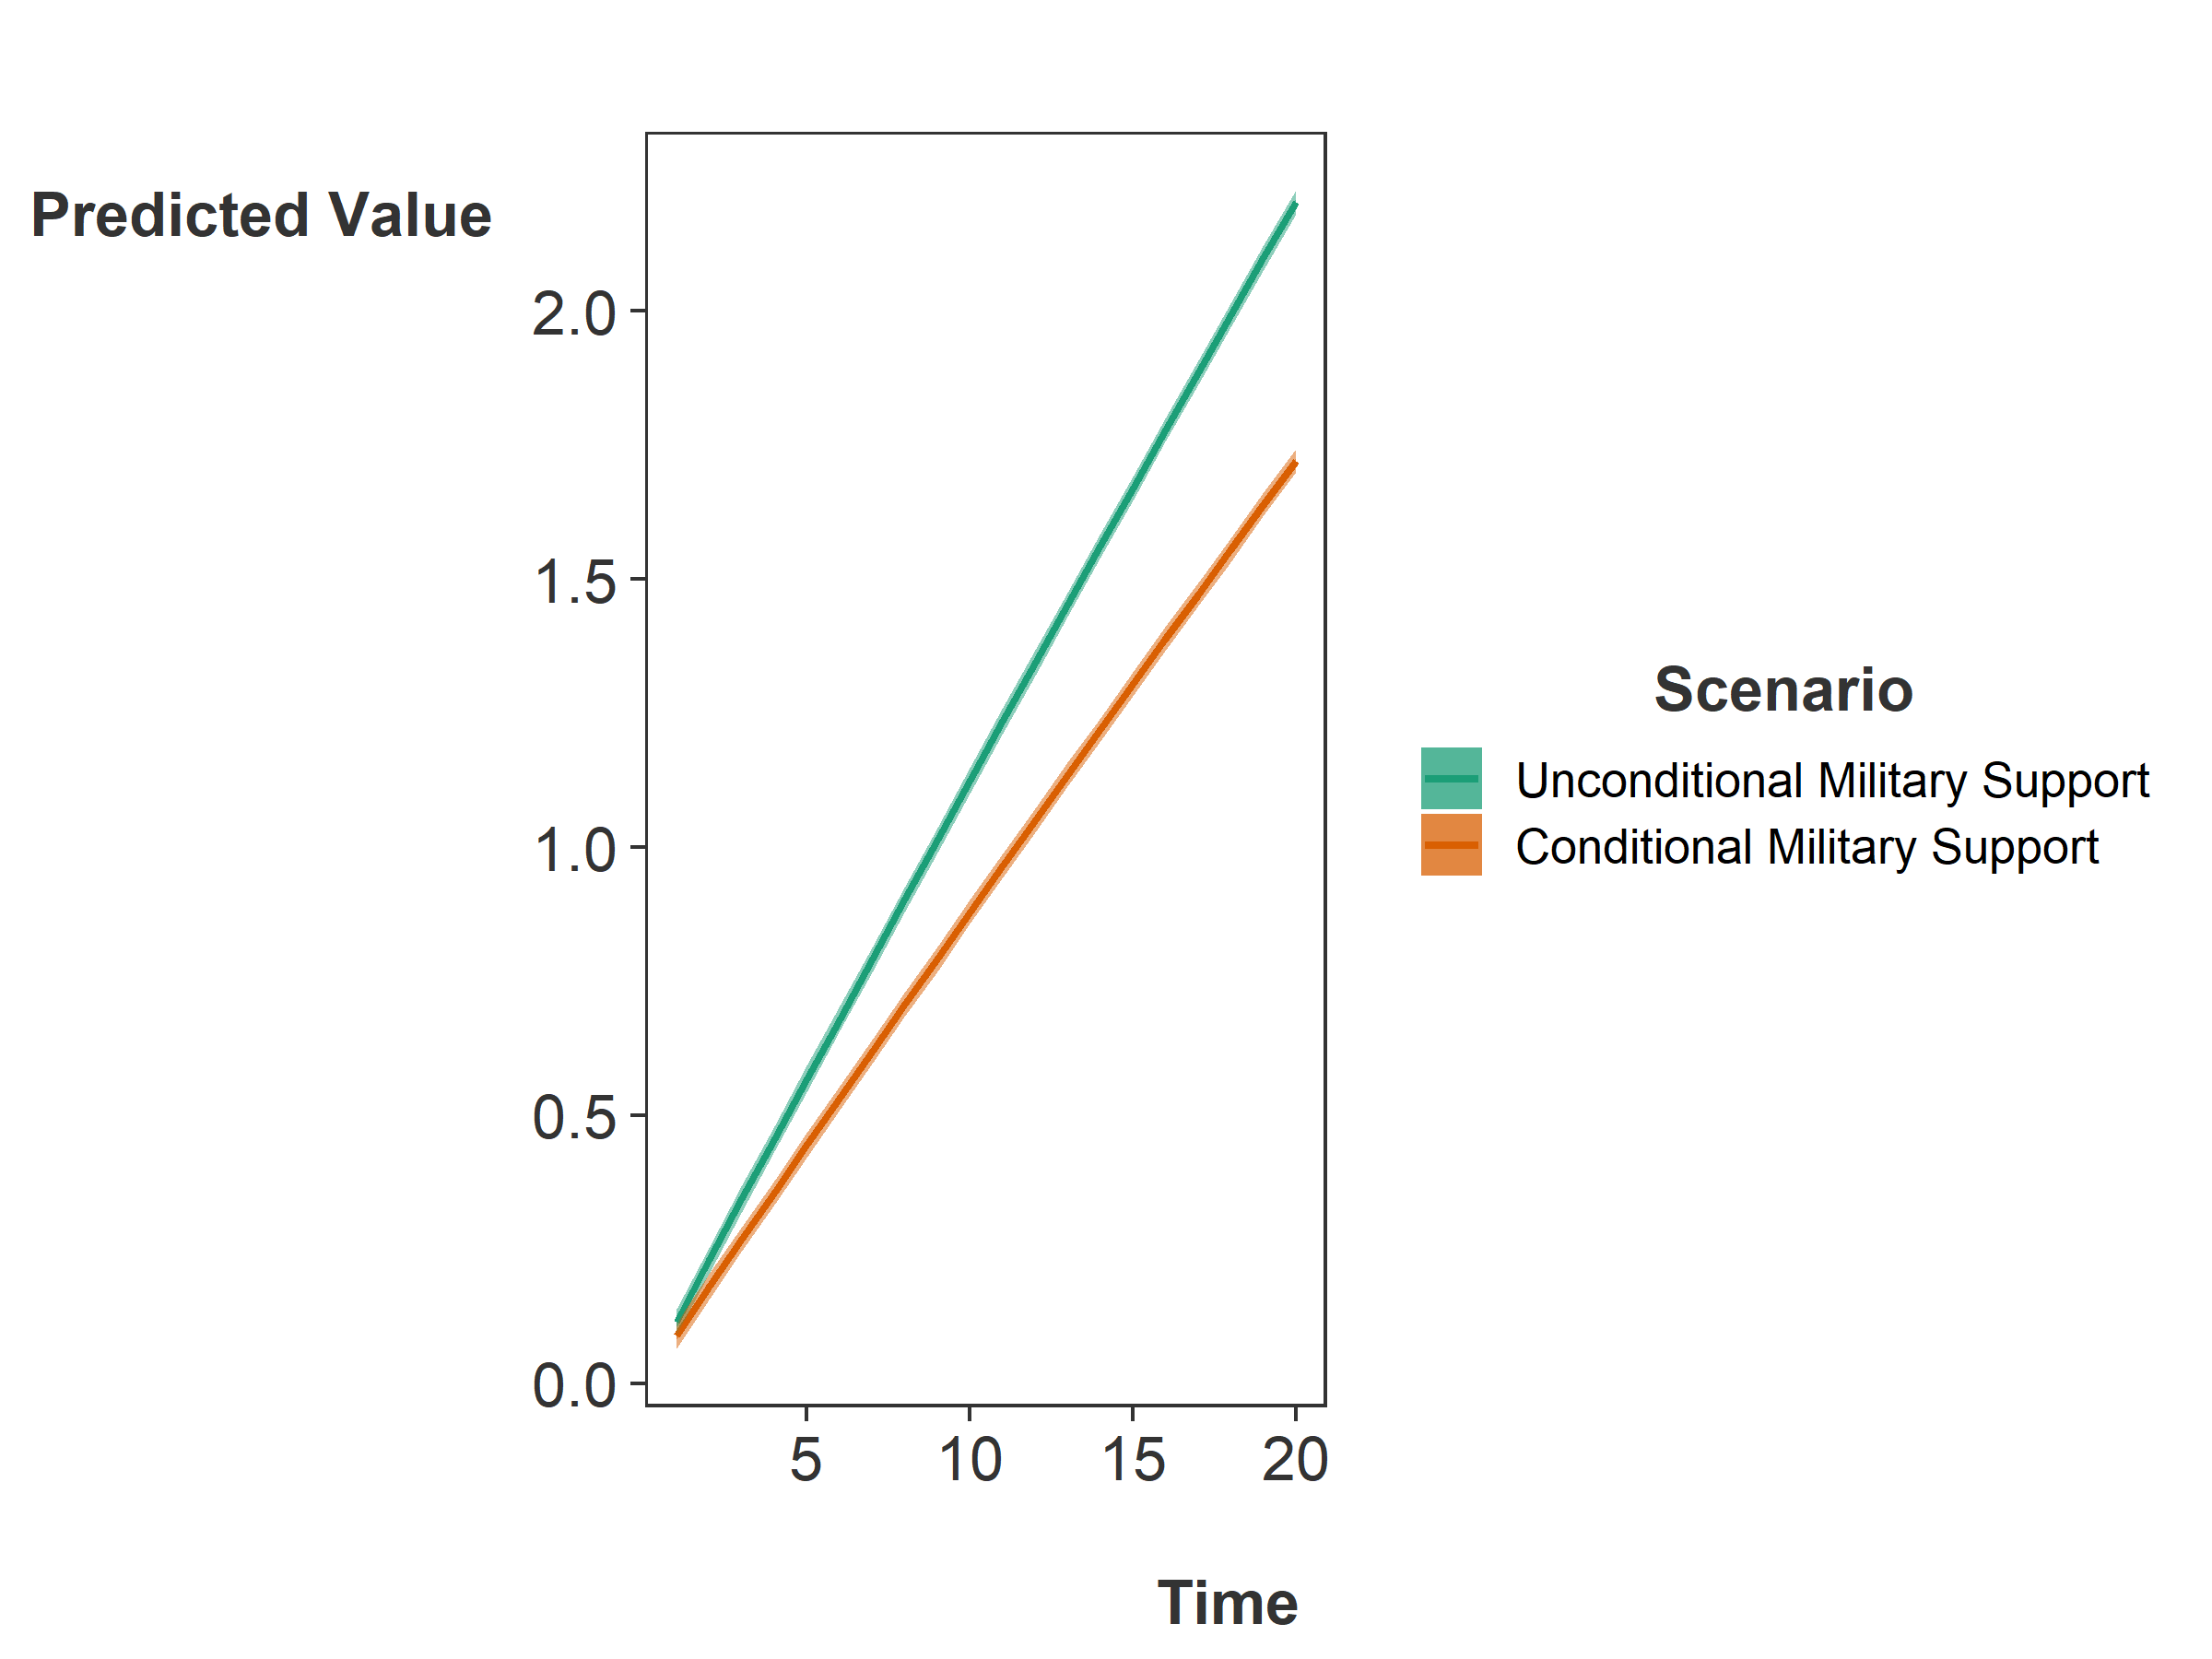
\includegraphics[width=0.99\textwidth]{mp-dynsim.png}
	\label{fig:mp-dynsim}
\end{figure}


\end{frame}



%-----------------------------------------------

\begin{frame}{Alternative Specifications} 

\begin{enumerate}
\item OLS.
\item FGLS.
\item Fixed Effects with Changes in Military Spending.  
\item Selection Models: Alliance Participants as Estimation Sample.
\item Multilevel Model with separate alliance-level regression. 
\end{enumerate}

\end{frame}

%------------------------------------------------

\section{Alternative Arguments}

%------------------------------------------------

\begin{frame}{(1) Value to Non-Major Powers} 

Strong commitments produce greater foreign policy gains. 

\pause

As a consequence, states are more willing to take costly actions to maintain the agreement. 


\end{frame}

%------------------------------------------------

\begin{frame}{Process}

\[
\begin{array}{ccccc}
\mbox{Alliance} &  \longrightarrow & \mbox{Foreign Policy} & \longrightarrow & \mbox{Assurance/} \\
\mbox{Formation} &                 & \mbox{Gains}     &                      & \mbox{Maintenance} 
\end{array}
\]


\end{frame} 

%------------------------------------------------

\begin{frame}{Alliance Member Size and Assurance}

Signal ongoing commitment through sunk costs.

\pause

Large states continue to bear the autonomy costs of strong commitments. %Imposing restraints on oneself is more costly/meaningful when actor is strong. 

\pause 

Smaller alliance partners increase military spending to signal ongoing commitment. 

\end{frame}



%------------------------------------------------

\begin{frame}{(2) Major Power Coercion} 

A different explanation emphasizes major power coercion of smaller partners. 
\pause

\begin{itemize}
\item Only form strong commitments with the expectation smaller partners will make significant contributions. 
\pause
\item Small states lose so much autonomy they must increase military spending. 
\end{itemize}


\end{frame}

%------------------------------------------------

\begin{frame}{Distinguishing Between Alternatives} 

There are a couple ways to distinguish between the two alternatives. 
\pause

\begin{enumerate}
\item Coercion: Smaller partner sacrifice autonomy on a range of other issues. 
\pause
\item Strong commitments reflect more hierarchical governance by larger partners. 
\end{enumerate} 

\end{frame}

%-----------------------------------------------

\section{Discussion and Conclusion}

%-----------------------------------------------

\begin{frame}{Discussion}

\pause 
Limitations:
\pause
\begin{enumerate}
\item Measurement error and missing data. 
\pause 
\item Alliances as military coalitions. 
\end{enumerate}

\end{frame}


%-----------------------------------------------

\begin{frame}{Conclusion}

Unconditional alliance treaties are associated with increased military spending by non-major powers.

\pause

Next Steps:
\pause
\begin{itemize}
\item Developing alternative arguments and considering when alliances decrease spending. 
\pause
\item More general measure of alliance treaty strength. 
\pause
\item Alternatives to major/non-major split. 
\end{itemize}

\end{frame}


%-----------------------------------------------

\appendix 

%------------------------------------------------


\begin{frame}{Regression Table}


\begin{table}
\begin{center}
\scalebox{.5}{
\begin{tabular}{l c c c }
\hline
 & Full Sample & Major Powers & Minor Powers \\
\hline
Unconditional Mil. Sup. & $0.03^{*}$        & $-0.02$           & $0.03^{*}$       \\
                   & $[0.01;\ 0.05]$   & $[-0.06;\ 0.03]$  & $[0.01;\ 0.06]$  \\
Conditional Mil. Sup.   & $0.01$            & $-0.00$           & $0.01$           \\
                   & $[-0.01;\ 0.03]$  & $[-0.04;\ 0.04]$  & $[-0.02;\ 0.03]$ \\
Lag ln(Mil. Ex.)       & $1.00^{*}$        & $1.00^{*}$        & $1.00^{*}$       \\
                   & $[0.99;\ 1.00]$   & $[0.99;\ 1.01]$   & $[0.99;\ 1.00]$  \\
At War             & $0.10^{*}$        & $0.11^{*}$        & $0.09^{*}$       \\
                   & $[0.08;\ 0.12]$   & $[0.09;\ 0.14]$   & $[0.06;\ 0.11]$  \\
Civil War Part.      & $0.01$            & $0.01$            & $0.01$           \\
                   & $[-0.00;\ 0.02]$  & $[-0.02;\ 0.04]$  & $[-0.00;\ 0.03]$ \\
Polity            & $0.00$            & $-0.00^{*}$       & $0.00$           \\
                   & $[-0.00;\ 0.00]$  & $[-0.01;\ -0.00]$ & $[-0.00;\ 0.00]$ \\
ln(GDP)            & $0.00$            & $0.02^{*}$        & $0.00$           \\
                   & $[-0.00;\ 0.00]$  & $[0.00;\ 0.03]$   & $[-0.00;\ 0.00]$ \\
Major Power          & $-0.03^{*}$       &                   &                  \\
                   & $[-0.04;\ -0.01]$ &                   &                  \\
External Threat           & $0.04^{*}$        & $0.07^{*}$        & $0.04^{*}$       \\
                   & $[0.02;\ 0.07]$   & $[0.01;\ 0.12]$   & $[0.02;\ 0.07]$  \\
Cold War          & $0.04^{*}$        & $0.00$            & $0.05^{*}$       \\
                   & $[0.04;\ 0.05]$   & $[-0.02;\ 0.03]$  & $[0.04;\ 0.06]$  \\
Avg Alliance Size        & $0.00$            & $0.00$            & $0.00$           \\
                   & $[-0.00;\ 0.00]$  & $[-0.00;\ 0.00]$  & $[-0.00;\ 0.00]$ \\
ln(Allied Spending)     & $-0.00$           & $-0.00$           & $-0.00$          \\
                   & $[-0.00;\ 0.00]$  & $[-0.01;\ 0.01]$  & $[-0.01;\ 0.00]$ \\
Avg Alliance Dem.      & $0.00$            & $0.00^{*}$        & $0.00$           \\
                   & $[-0.00;\ 0.00]$  & $[0.00;\ 0.01]$   & $[-0.00;\ 0.00]$ \\
Constant       & $0.04^{*}$        & $-0.44^{*}$       & $0.05^{*}$       \\
                   & $[0.01;\ 0.07]$   & $[-0.76;\ -0.13]$ & $[0.01;\ 0.08]$  \\									
\hline
Num. obs.          & 9461              & 916               & 8545             \\
\hline
\multicolumn{4}{l}{\scriptsize{$^*$ 0 outside the confidence interval}}
\end{tabular}
}
\label{table:coefficients}
\end{center}
\end{table}


\end{frame}

%-----------------------------------------------

\begin{frame}{ML Model Results}


\begin{figure}
	\centering
		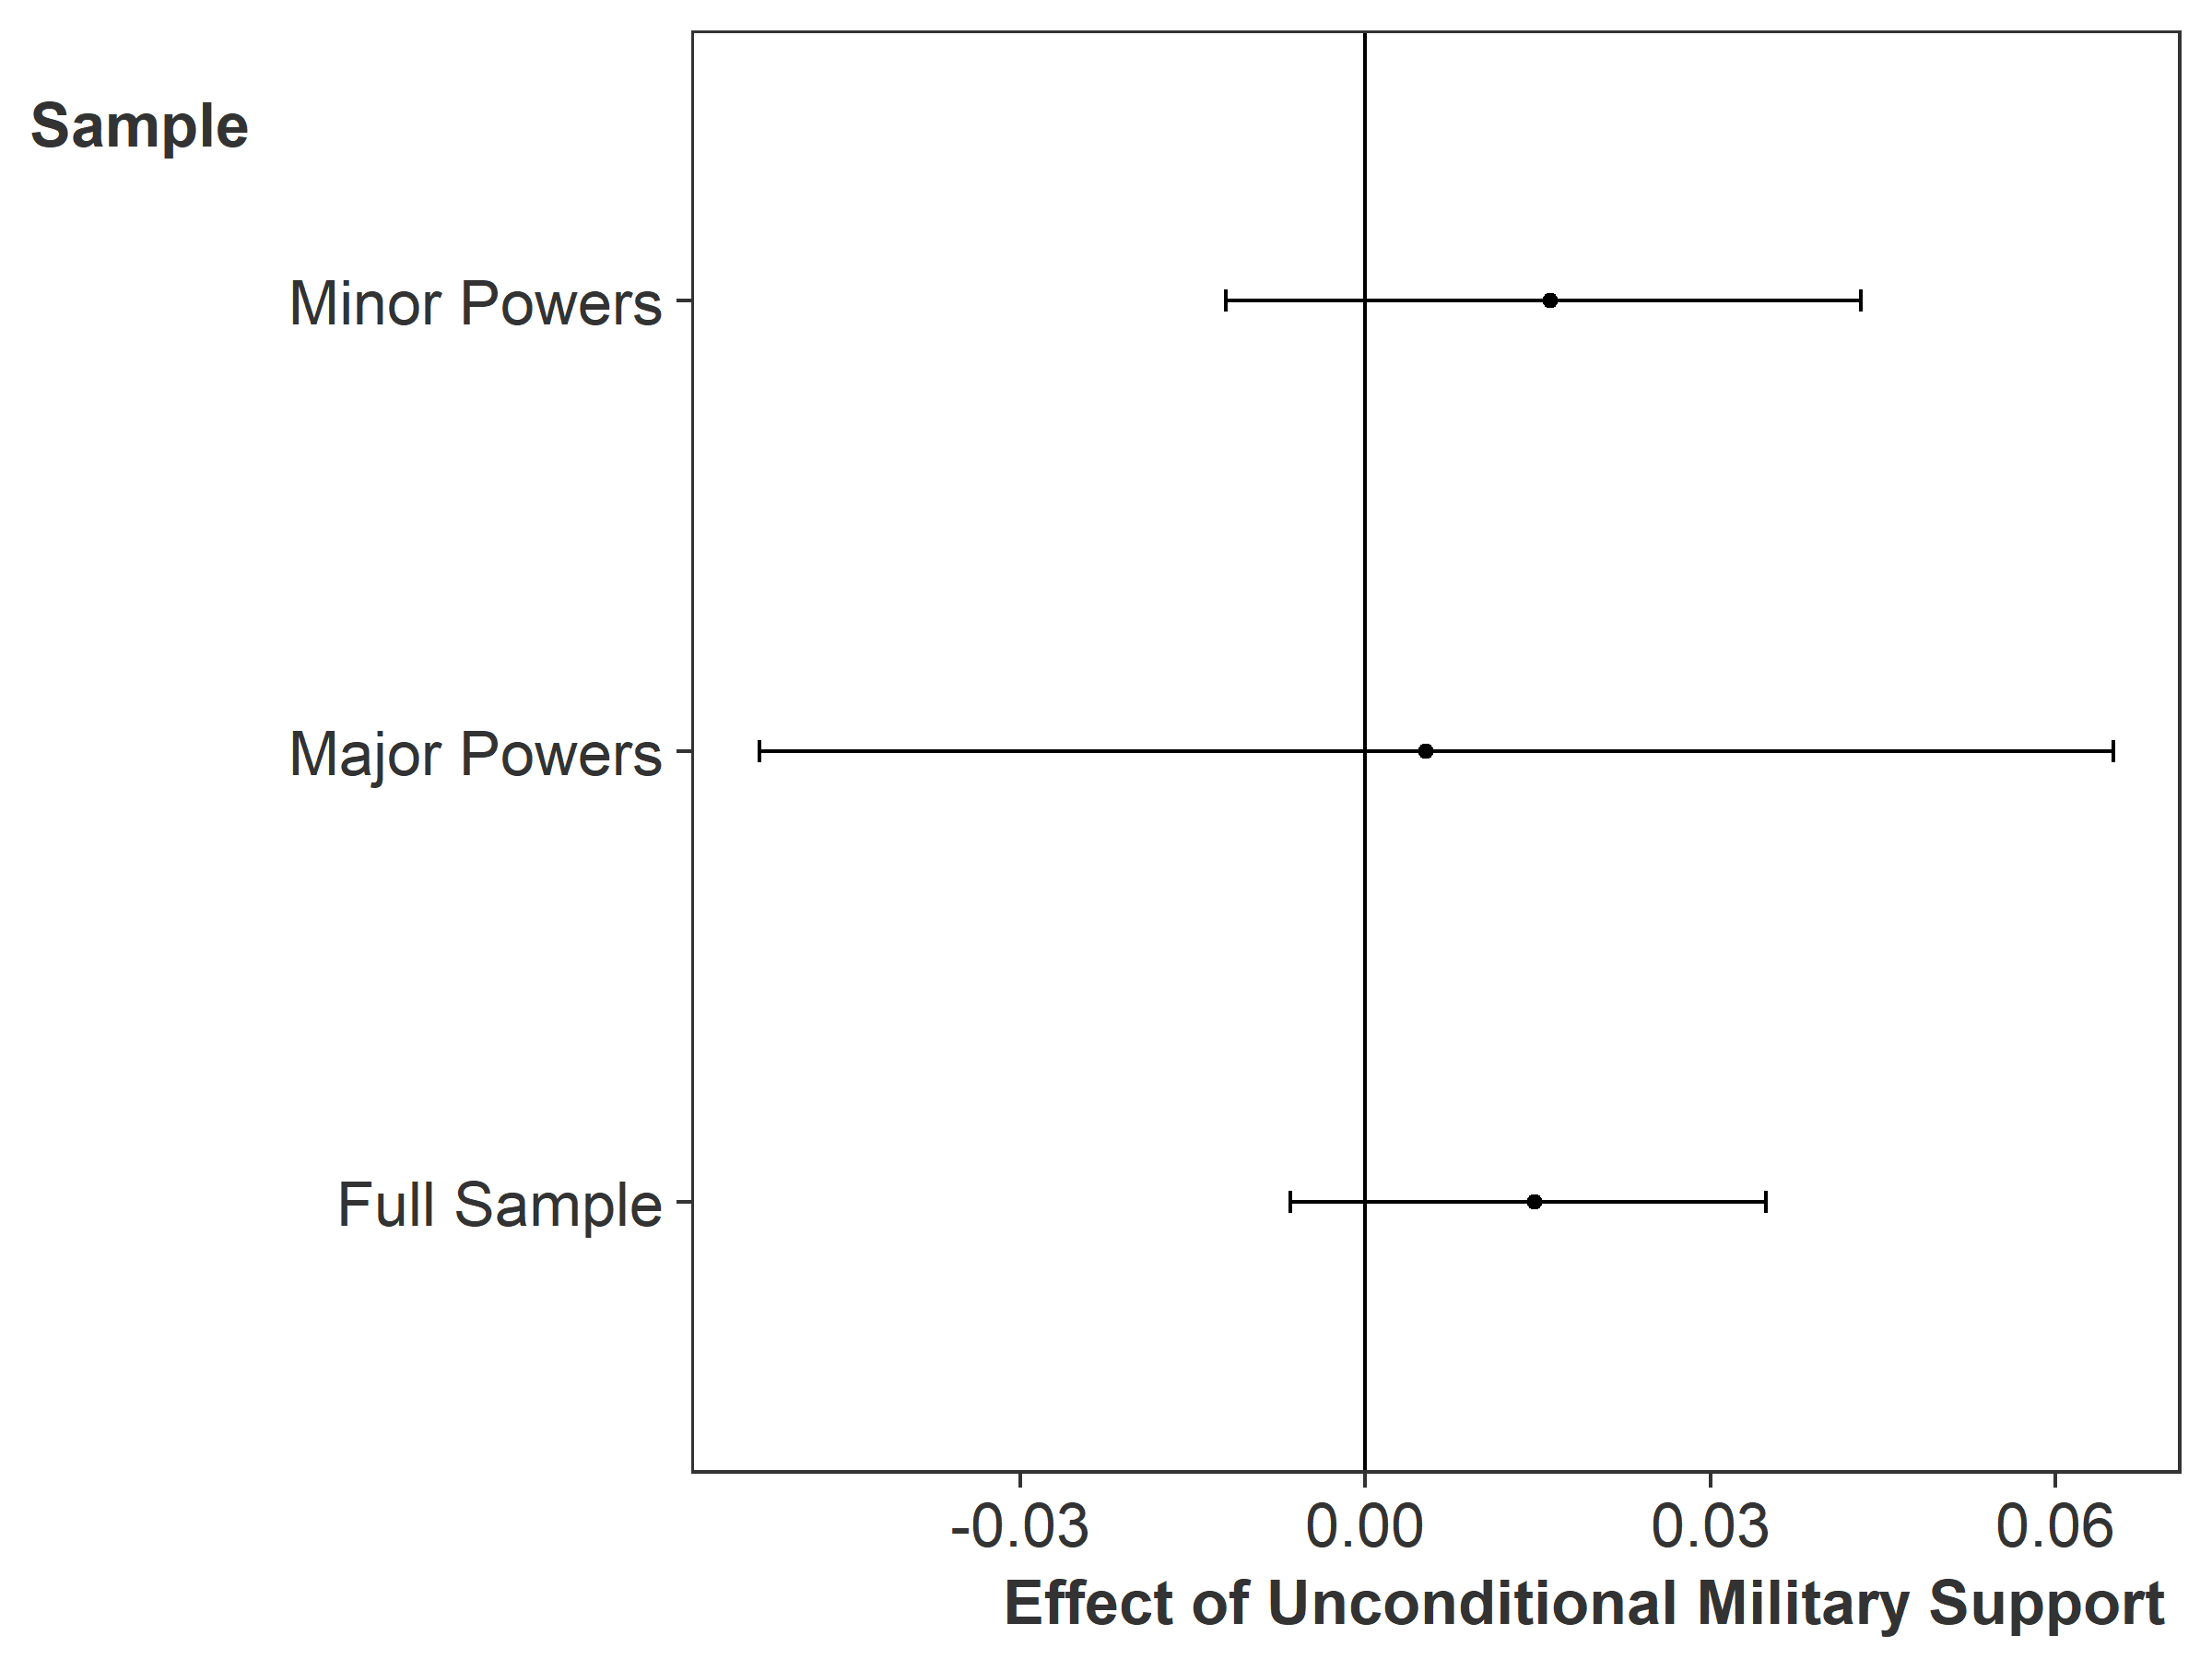
\includegraphics[width=0.95\textwidth]{ml-model-uncond-coefs.png}
	\label{fig:ml-model-uncond-coefs}
\end{figure}


\end{frame}


%------------------------------------------------


\begin{frame}{Priors}

\begin{table} % Create a table of priors.

 \begin{center}
\begin{tabular}{c} 
$ p(\alpha) \sim N(0, 3)$  \\
$ p(\sigma) \sim \mbox{half-}N(0, 1) $ \\
$ p(\alpha^{yr}) \sim N(0, \sigma^{yr}) $ \\ 
$ p(\sigma^{yr}) \sim N(0, 1) $ \\
$ p(\alpha^{st}) \sim N(0, \sigma^{st}) $ \\ 
$ p(\sigma^{st}) \sim \mbox{half-}N(0, 1) $ \\ 
$ p(\sigma^{all}) \sim \mbox{half-}N(0, 1) $ \\
$ p(\eta) \sim \mbox{half-}N(0, 1) $ \\
$ p(\beta) \sim N(0, 1) $ \\
$ p(\gamma) \sim N(0, 1) $ \\ 
$ p(\nu) \sim gamma(2, 0.1)$ 
\end{tabular} 
\end{center} 
\label{tab:priors}
\end{table} 


\end{frame}

%------------------------------------------------

\begin{frame}{Positive Posterior Probability of all Coefficients}

\begin{figure}
	\centering
		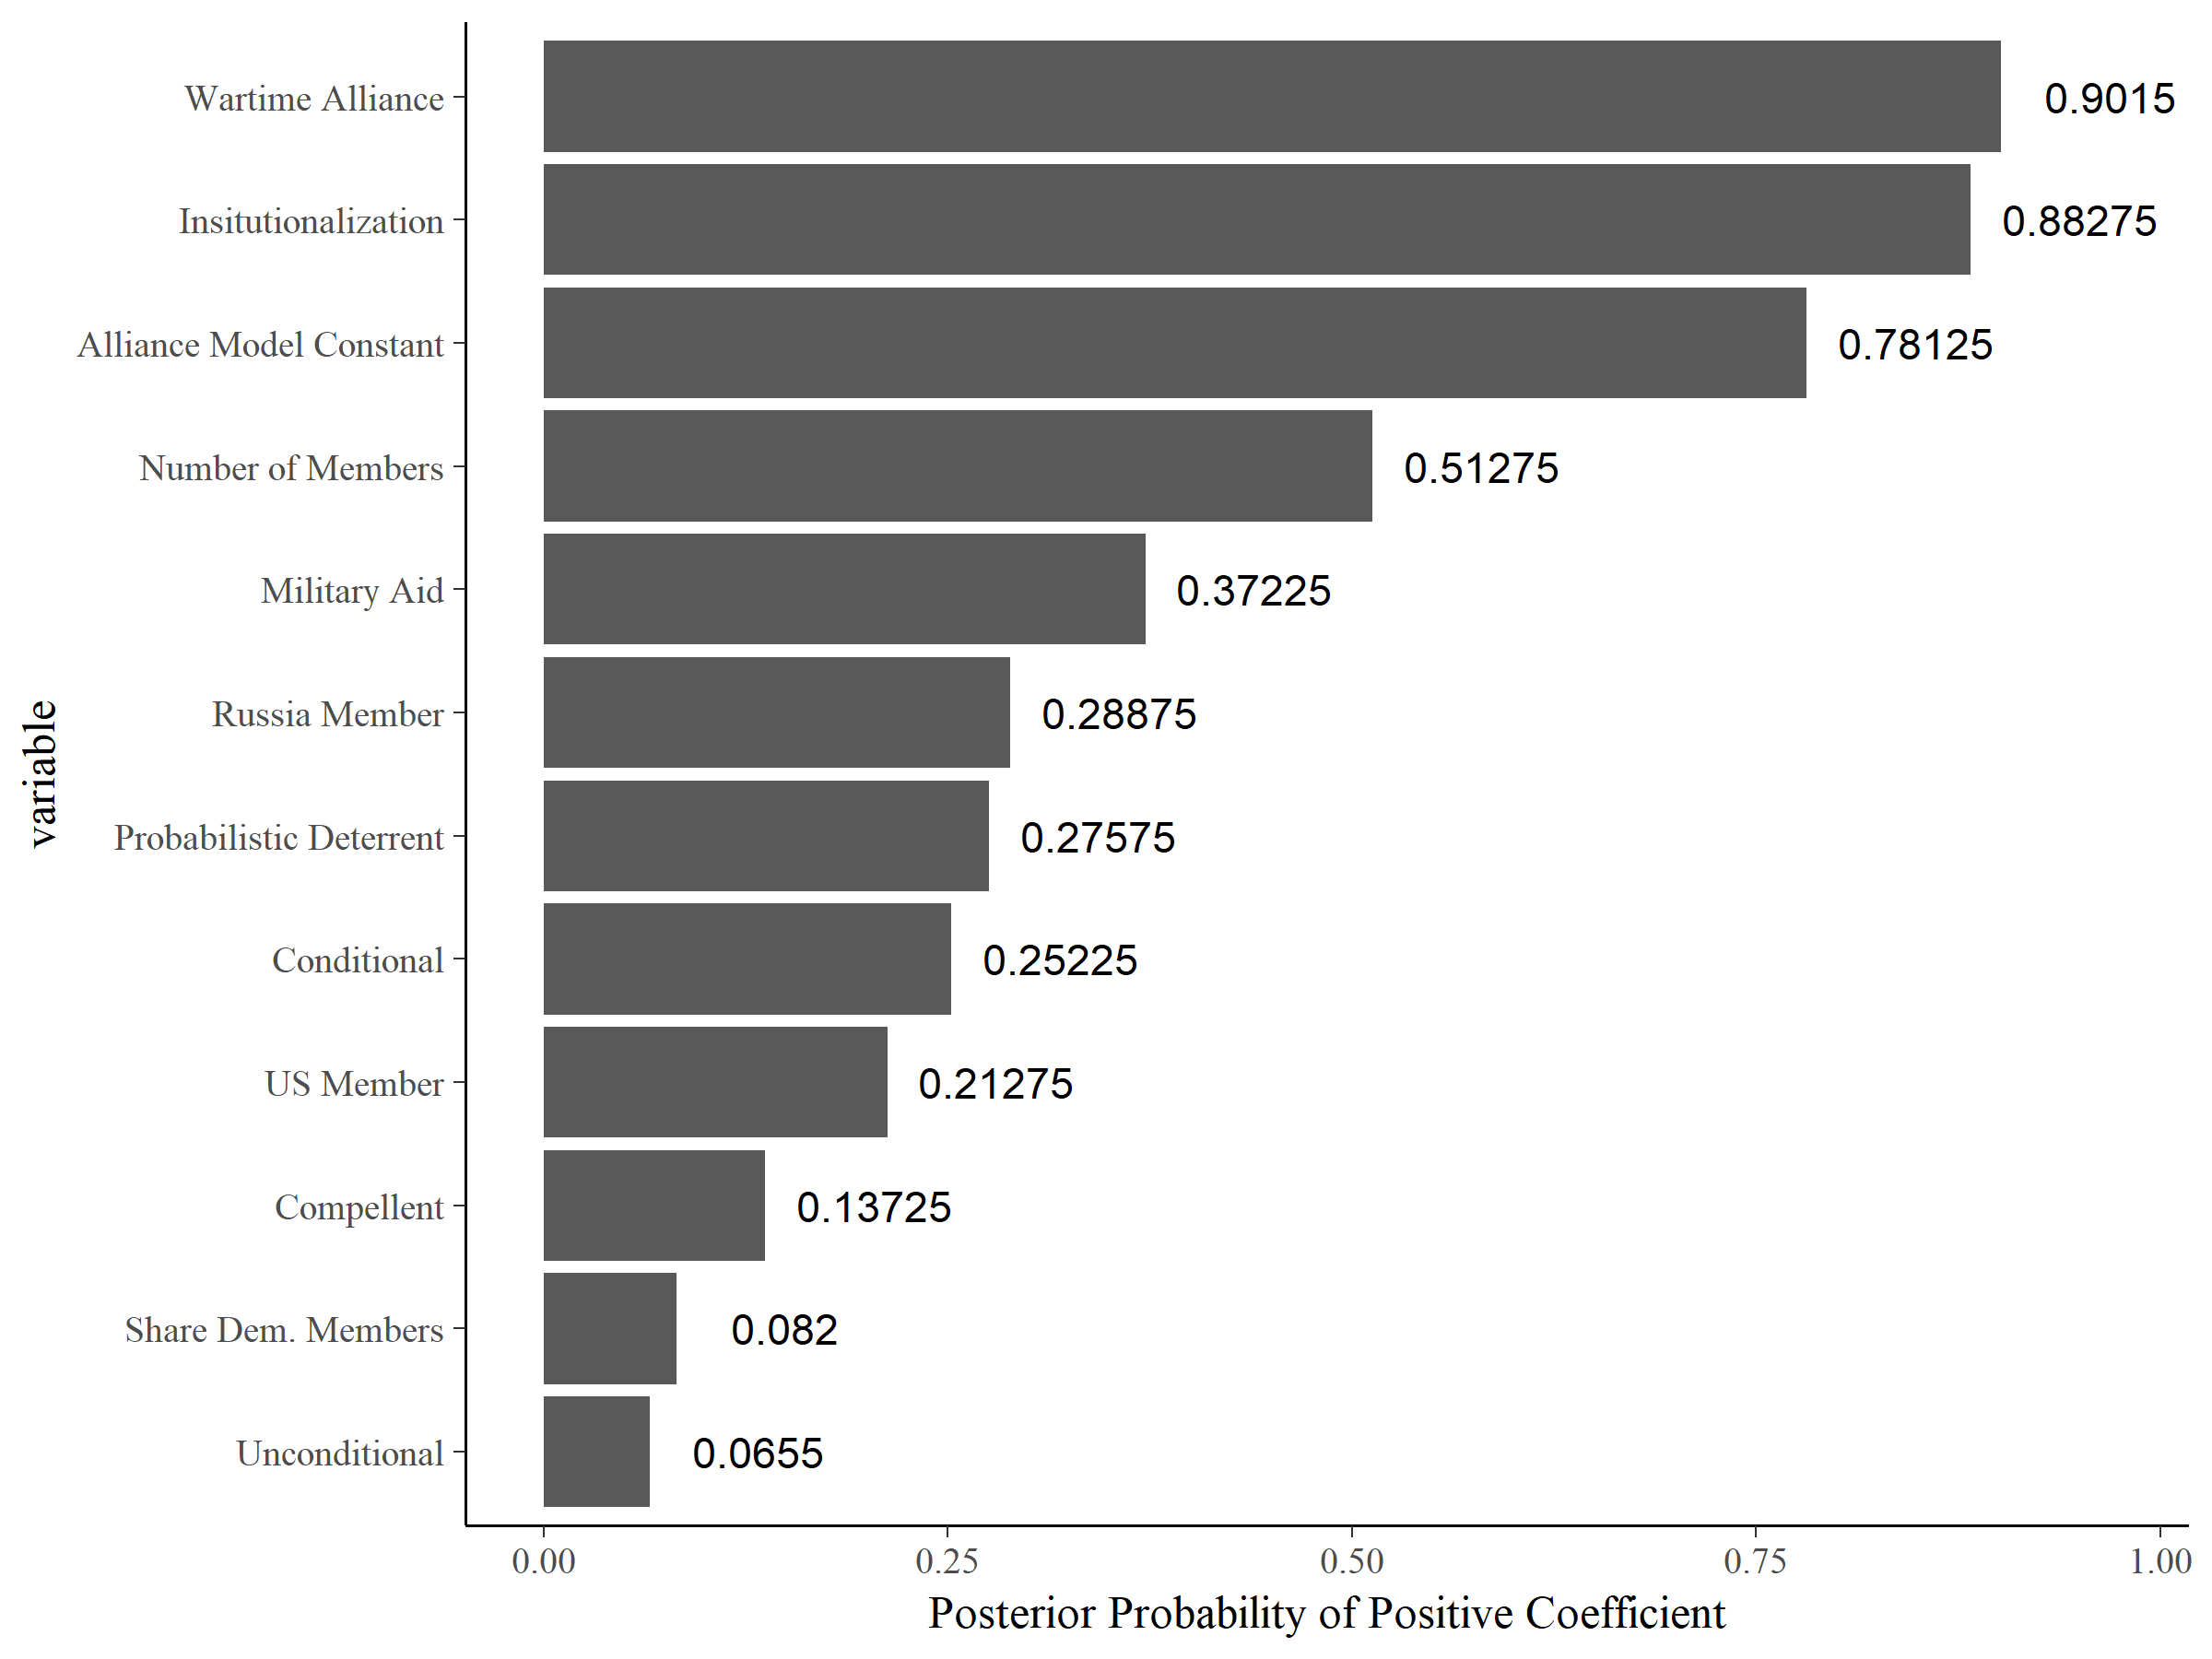
\includegraphics[width=0.95\textwidth]{post-prob-beta.png}
	\label{fig:post-prob-beta}
\end{figure}


\end{frame}

%------------------------------------------------

\begin{frame}{Non-zero alliances}

\begin{figure}
	\centering
		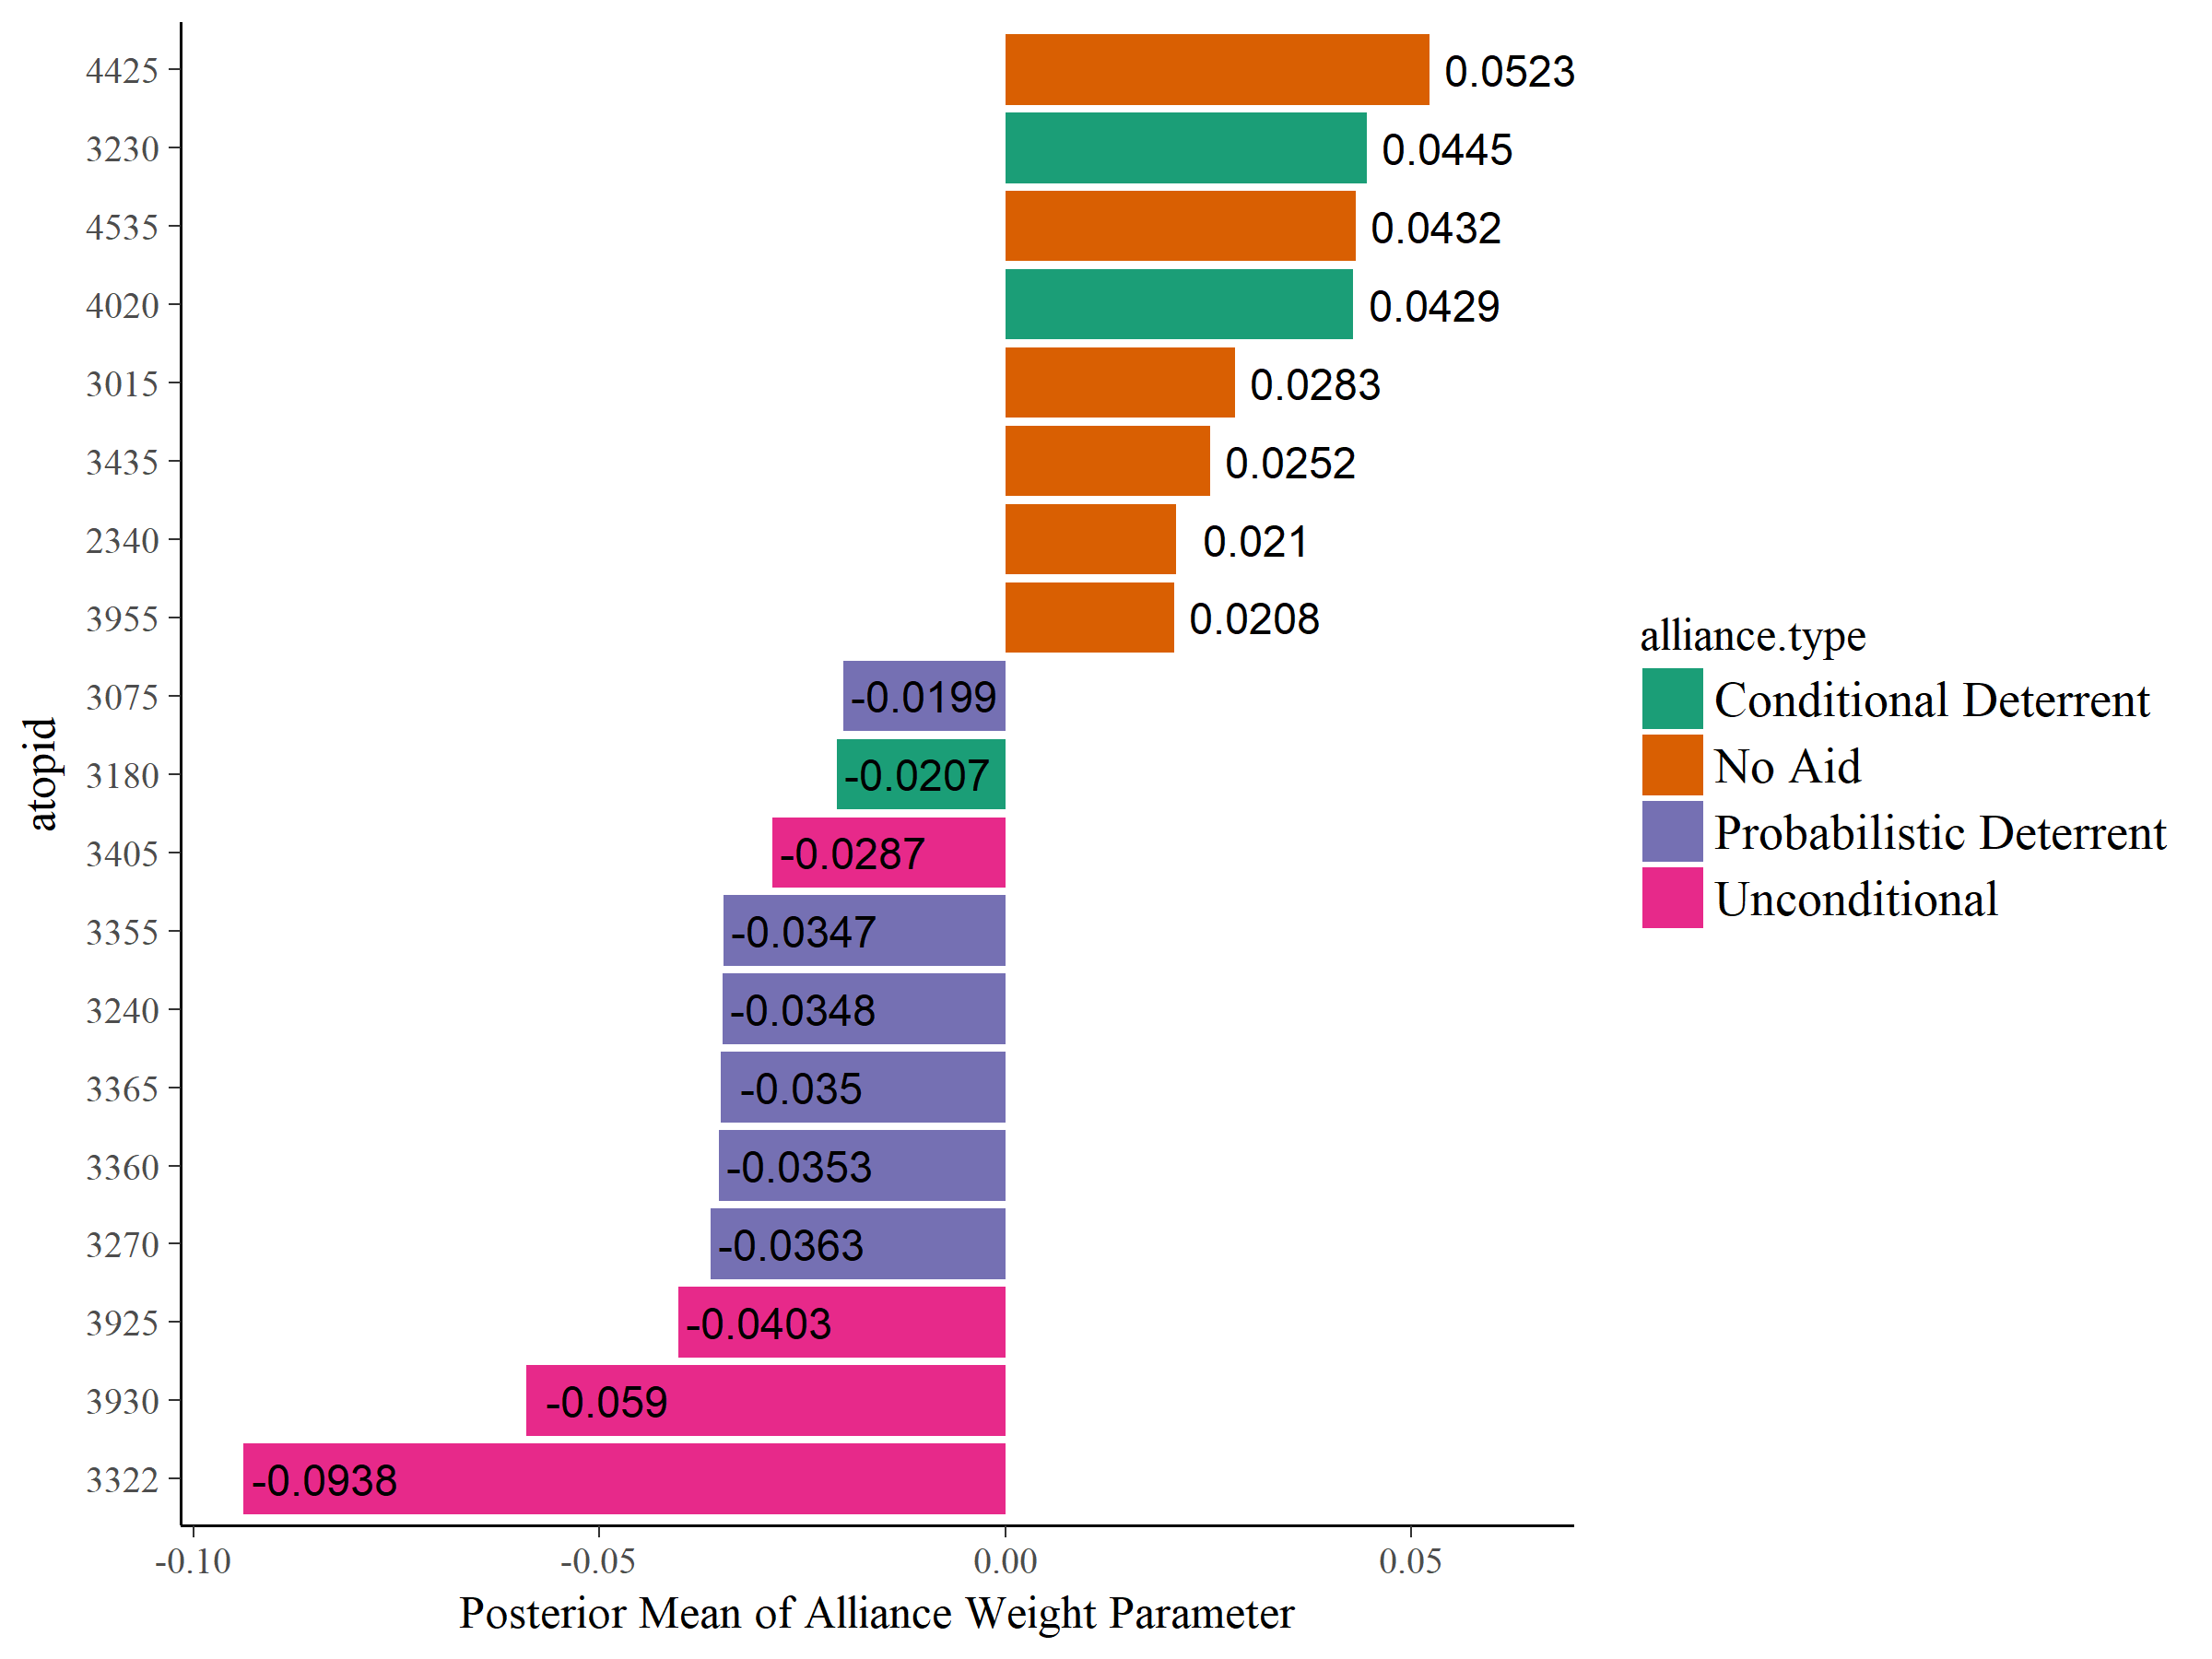
\includegraphics[width=0.95\textwidth]{non-zero alliances.png}
	\label{fig:non-zero alliances}
\end{figure}


\end{frame}

%------------------------------------------------

\begin{frame}{Violin Plot of Mean $\lambda$ for all alliances}

\begin{figure}
	\centering
		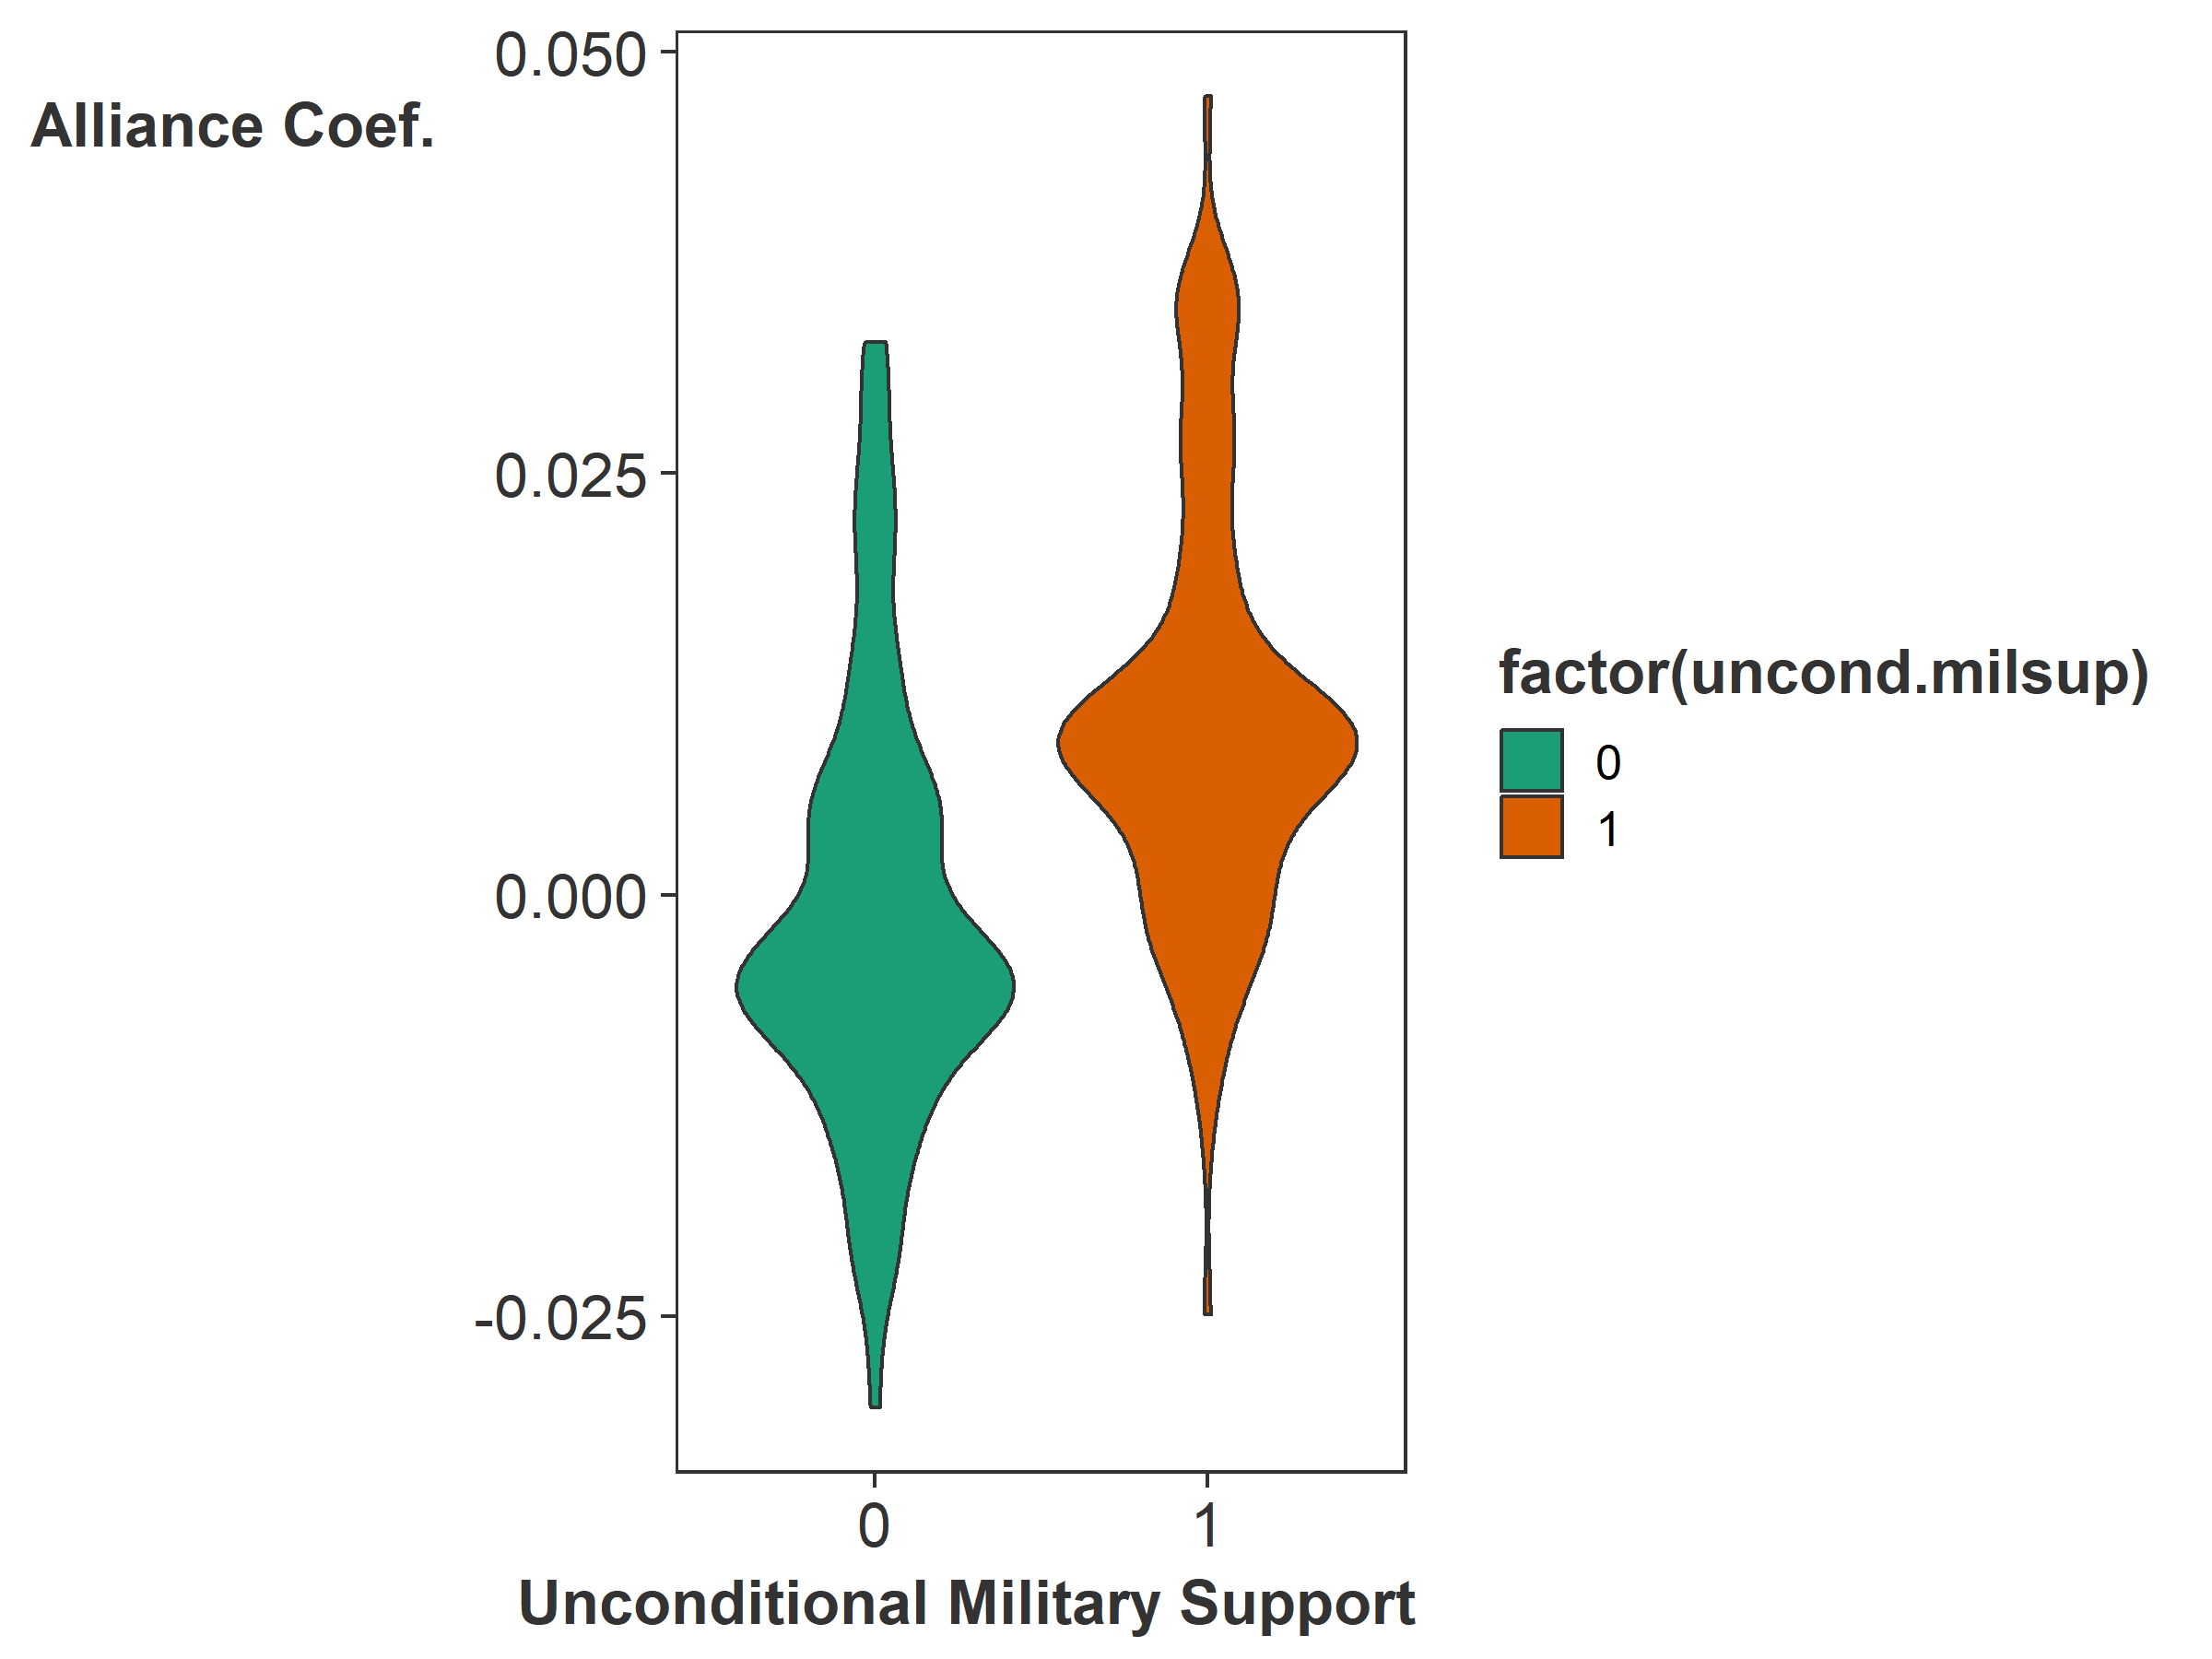
\includegraphics[width=0.95\textwidth]{lambda-box-presentation.png}
	\label{fig:lambda-box-presentation}
\end{figure}


\end{frame}


%----------------------------------------------------------------------------------------

\end{document}